\section{Test af hardware}
\subsection{Modultest}
Før at vi kunne teste det samlede system bestående af både hardware og software, måtte vi foretage nogle modultests af de enkelte dele i hardwaren. Forstærkeren, subtractoren samt antialiaseringsfilteret er blevet testet på fumlebrættet, og i forbindelse med disse test har vi skiftet mellem at bruge en spændingsdeler og en tryktransducer som var tilsluttet vandsøjlen. Da testene var godkendt, kunne vi tilkoble alt hardwaren og lave integrationstest.


\subsubsection{Forstærker}
I testen for forstærkeren brugte vi en spændingsdeler, da Analog Discovery ikke kan levere en lav nok spænding uden at være påvirket af støj. Spændingsdelerens skulle levere en lav spænding på 12,5 mV eller lavere, da transducerens output tilsvarende er en lav spænding. De 12,5 mV er beregnet under design afsnittet for forstærkeren. Spændingsdeleren fungerede derfor som en erstatning af transduceren, hvor vi blot selv kunne bestemme hvilket type signal vi ville sende igennem forstærkeren.

\textbf{Test med spændningsdeler}

For at teste om signalet blev forstærket 320 gange af forstærkeren, sendte vi 4 V gennem spændingsdeleren og forstærkeren, og målte på udgangen af forstærkeren. Spændingsdeleren var i denne test designet til at kunne levere et output svarende til 320 gange mindre end 4 V, hvilket svarer til 12,5 mV, som er transducerens max output. Denne viden kunne vi benytte, så inputtet til spændingsdeleren og outputtet fra forstærkeren burde være det samme.

Da vi målte på udgangen af forstærkeren, fik vi et en spænding på 4 V, hvilket stemte overens med vores forventede resultater.


\textbf{Test med transducer og vandsøjle}

I denne test erstattede vi spændingsdeleren med transduceren, som blev tilsluttet vandsøjlen. Der blev udført en række tests med forskellige tryk på transduceren, for at undersøge om signalet blev forstærket op 320 gange, samt teste lineariteten og nøjagtigheden af vores målinger.

Nedenstående graf repræsenterer testresultaterne fra et tryk på 0, 10, 50 og 100 mmHg.


\vspace{0.5 cm}

\begin{figure}[h!]
	\centering
	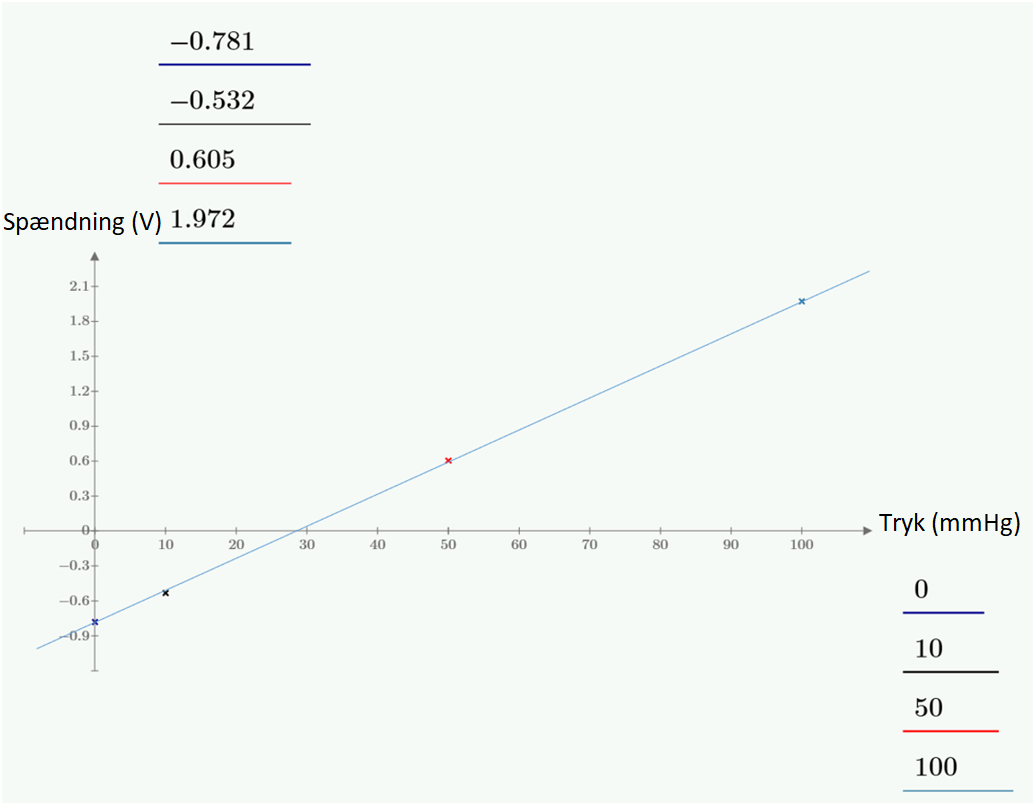
\includegraphics[width=0.6\linewidth]{../Rapport/Implementering_og_test/Hardware/forstaerker}
	\caption{Spænding som funktion af tryk}
	\label{fig:forstaerker}
\end{figure}

\clearpage

På x-aksen er tryk i mmHg, og på y-asken er spænding i V. Det ses at der er en god lineær sammenhæng mellem tryk og spænding, samt at signalet er blevet forstærket. Da vi på vandsøjlen kun kan måle op til 100 mmHg antager vi at denne sammenhæng fortsætter, og kan opstille følgende regnestykke: 

\[\frac{250 mmHg}{100 mmHg} = 2,5 \]
\[ 1,972 V \cdot 2,5 = 4,93 V \]
\[ 4,93 V - 0,781 V = 4,149 V \]

Ovenstående værdier kommer fra figur \textbf{X}, hvor de 1,972 V er spændingen ved 100 mmHg. De 4,93 V er den forventede spænding ved 250 mmHg, hvor det atmosfæriske tryk er inkluderet. For at finde den korrekte værdi for 250 mmHg uden atmosfærisk tryk trækkes de 0,781 V fra, hvilket er skæringen med y-aksen, som på denne graf er tilsvarende det atmosfæriske tryk. Da vores antagelser ligger udenfor det målbare område er det regnestykket ekstrapolært, og er dermed forbundet med en større usikkerhed.

Ud fra tidligere beregninger vil vi forvente at et tryk på 250 mmHg vil have en spænding på 4 V, hvilket stemmer godt overens med vores test. De specifikke måleresultater findes i bilag for test af hardwaren.

\subsubsection{Subtractor}

For at teste subtractoren brugte vi waveforms til at genere to signaler. Et DC-signal på 2 V, hvilket subtractoren bruger til at trække et signal ned med 2 V. Det andet signal var et sinussignal, som blev sendt gennem subtractoren. I testen forventede vi, at subtractoren ville sænke sinussignalet 2 V ned i dens amplitude. Vi sendte et sinussignal ind med et offset på 2 V, for at hæve signalet, som vi derefter vha. subtractoren kunne sænke. Vi målte signalerne ved brug af waveforms scope funktion.

\begin{figure}[h!]
	\centering
	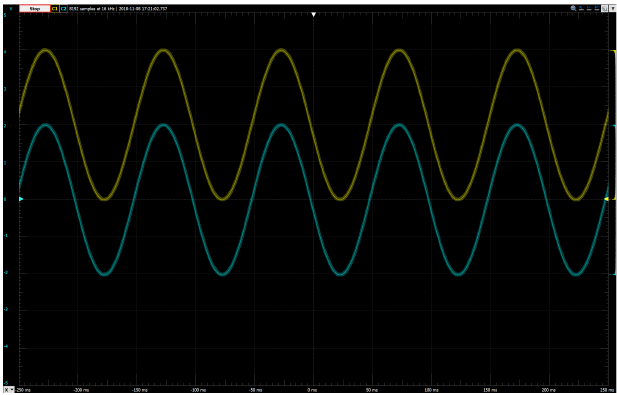
\includegraphics[width=0.72\linewidth]{../Rapport/Implementering_og_test/Hardware/subtractor}
	\caption{Test af subtractor. På y-aksen ses spændning (V), og på x-aksen ses tid (sekunder)}
	\label{fig:subtractor}
\end{figure}

På ovenstående screenshot ses den gule kurve, som et sinussignal med en amplitude på 2 V og et offset på 2 V. Der benyttes et sinussignal, for at teste subtractorens nedeskalering af forskellige amplituder. Den blå kurve er outputtet fra subtractoren, hvilket har sænket det oprindelige sinussignal med 2 V.

Subtractoren virkede derfor som den skulle, i og med at den kunne sænke signalet med de ønskede 2 V.


\subsubsection{Filter}

Da vi testede filteret, sendte vi et sinussignal ind på filteret med en amplitude på 2 V. For at undersøge filtrets dæmpning gav vi signalet 24 forskellige hertz i et range på 10 til 500 Hz. Resultaterne er påvist på nedenstående bodeplot.

\begin{figure}[h!]
	\centering
	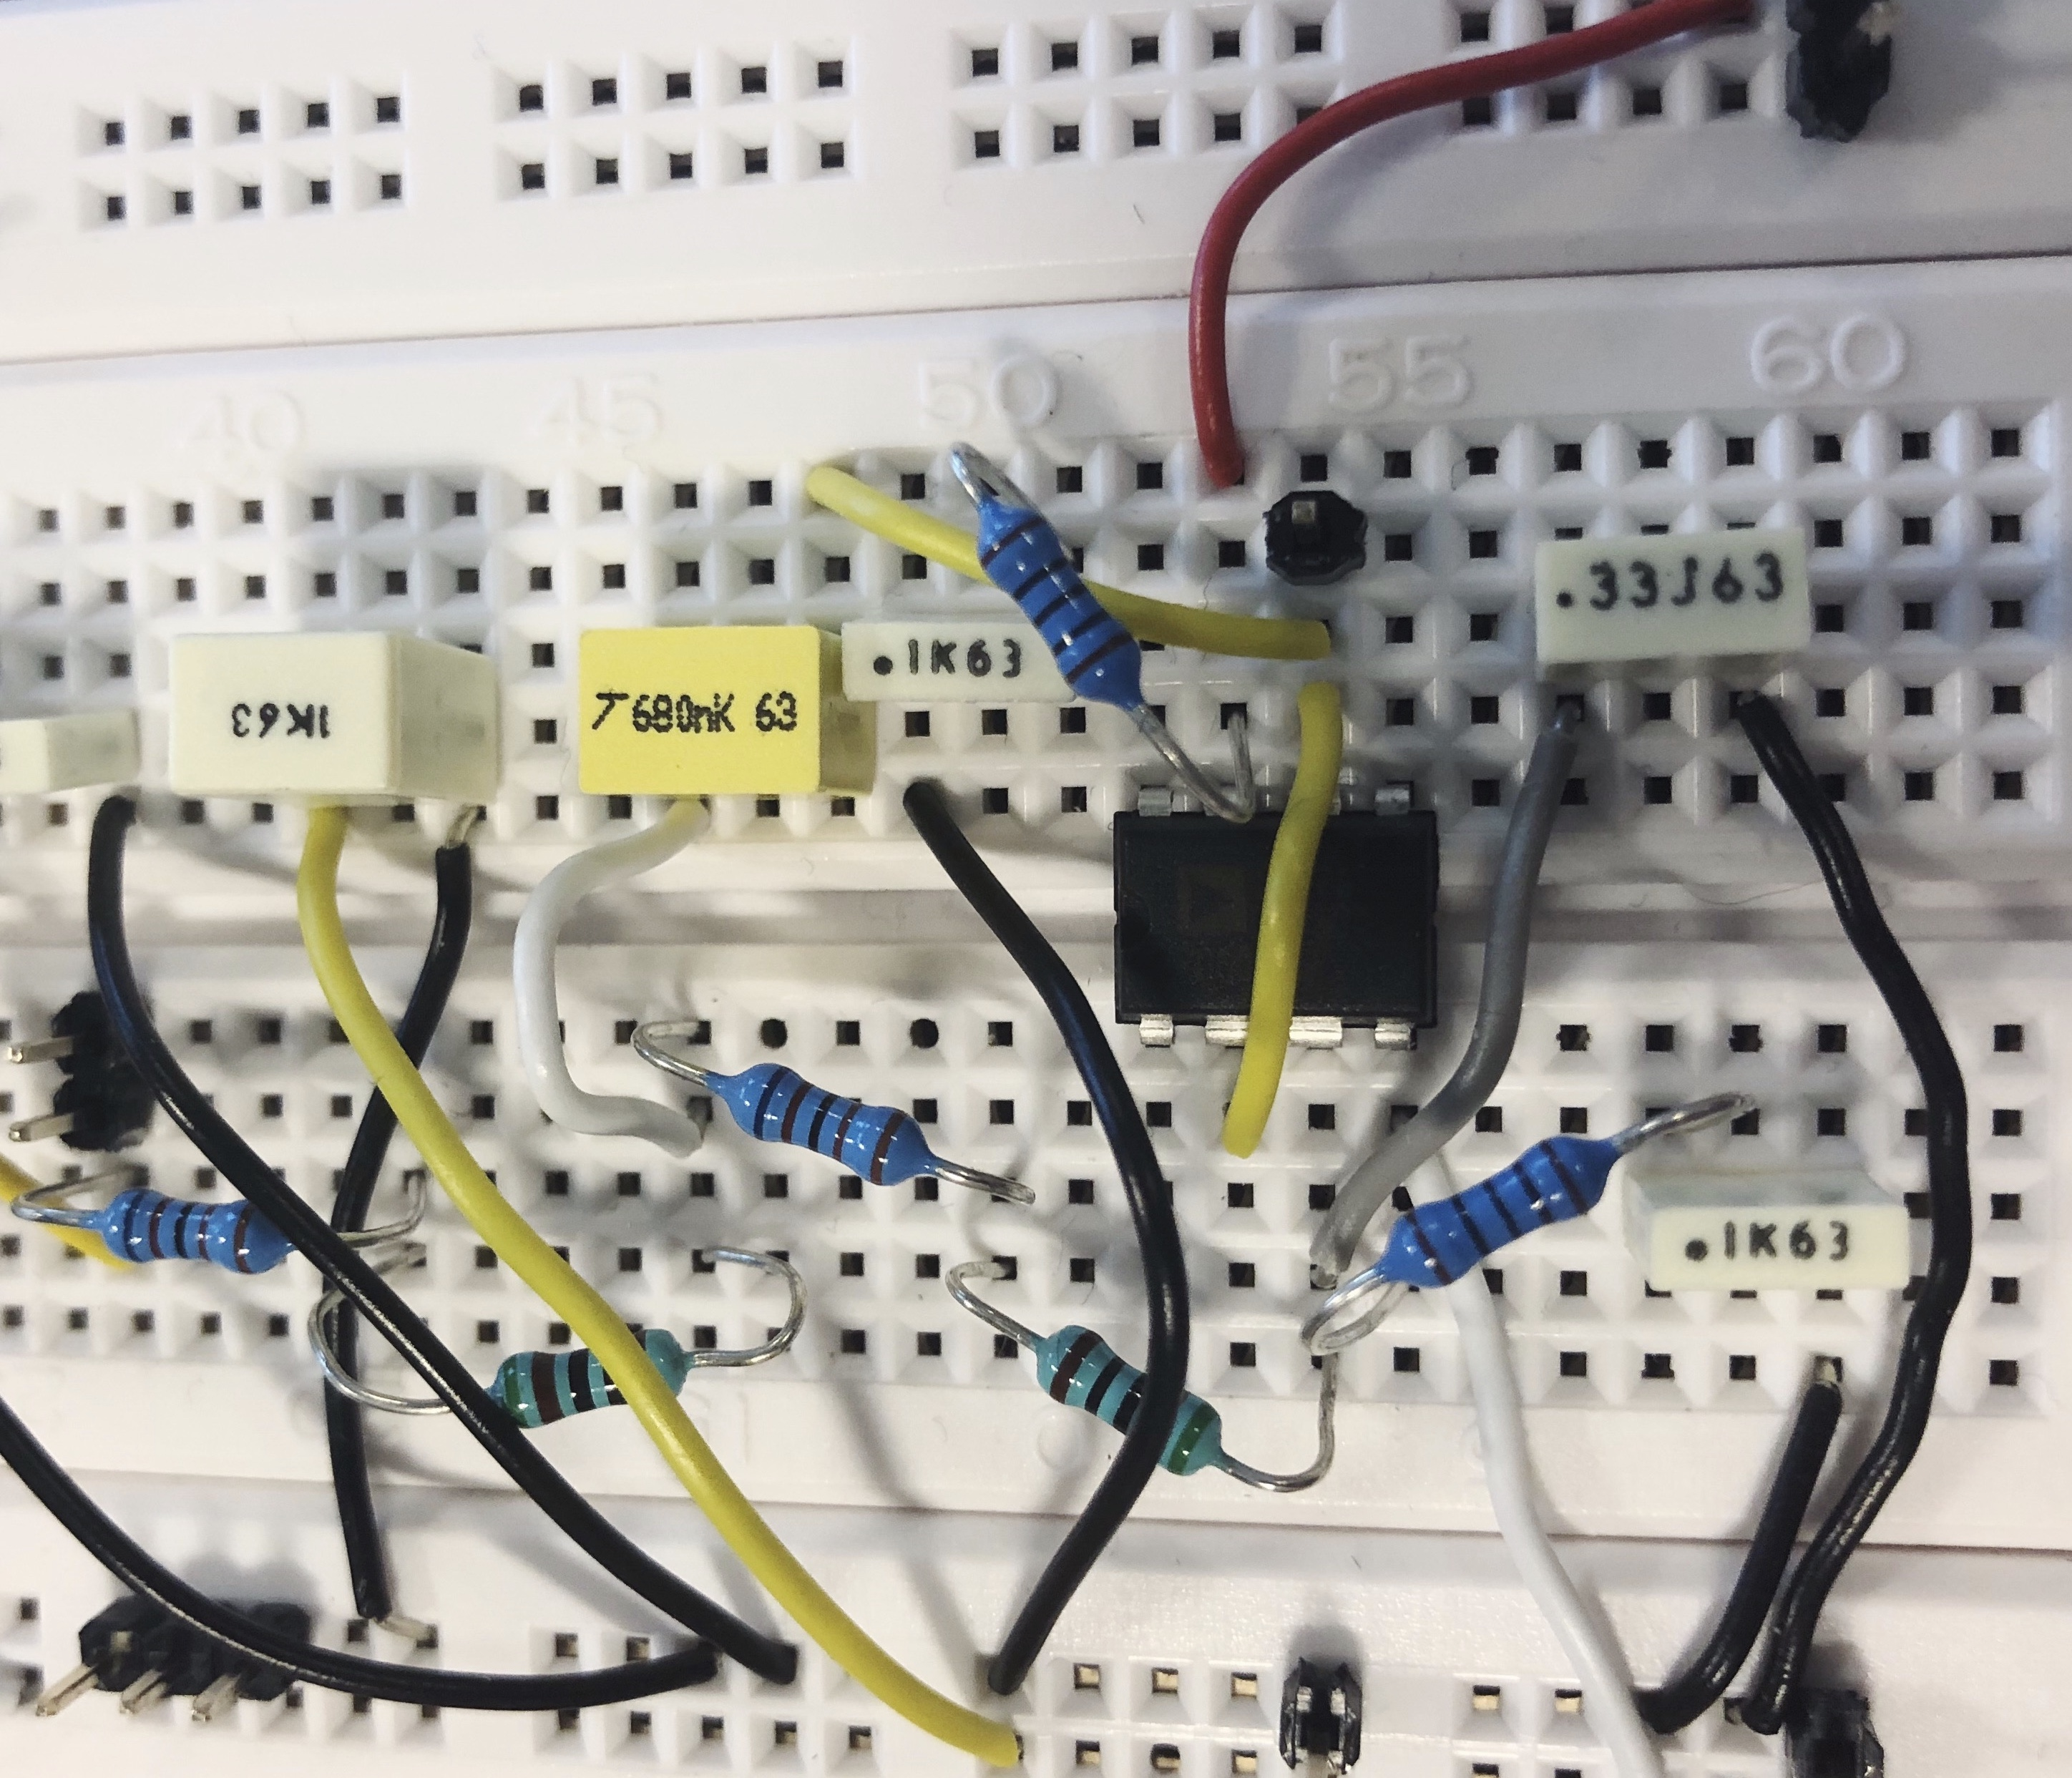
\includegraphics[width=0.8\linewidth]{../Rapport/Implementering_og_test/Hardware/filter2}
	\caption{Bodeplot af 2. ordens antialiaseringsfilteret}
	\label{fig:filter}
\end{figure}

Knækfrekvensen er påtegnet som den sorte vertikale linje på figur X, hvilket er det fjerde målepunkt på grafen, som er 50 Hz. Filteret har allerede ved 50 Hz har sænket signalet med -3 dB, hvilket skyldes at filterets dæmpningsfaktor er 0,707, som giver det fladeste bodeplot. Tager man 20*log(0,707) fås der tilsvarende en værdi på -3 dB.

Det ses at signalet dæmper 40 dB pr dekade, hvilket stemmer overens med vores ventede resultat. De specifikke måleværdier kan findes i bilag for test af hardwaren.

Kravet er at filteret skal dæmpe 20 dB over den dekade der er til rådighed, så i teorien har vi ikke brug for et 2. ordensfilter. Dog i tilfælde af at vi brugte 1. ordensfilter, skulle alt performe fuldstændigt perfekt, hvilket var en risiko vi ikke var villige at tage, og derfor benytter vi et 2. ordensfilter.

\clearpage

\subsubsection{Integrationstest med vandsøjle}

Da modulttestene var gennemført med tilfredsstillelse, blev hele systemet sammenkoblet, således der kunne laves en integrationstest for hele systemet. Formålet med denne test er at undersøge, om hele systemet kan integrere fornuftigt med hinanden, samt undersøge hvilke output de forskellige tryk på vandsøjlen giver, og dermed finde en sammenhæng mellem tryk og spænding.
Der blev testet ved 5 forskellige tryk, hvilke var 0, 10, 25, 50, 75 og 100 mmHg. Vi forventede at få en talrække indenfor -2 V og 2 V, da forstærkeren burde forstærke op i et spænd fra 0-4 V, og subtractoren herefter ville sænke signalet med 2 V.

Resultaterene fra testen er blevet plottet på nedenstående figur:

\begin{figure}[h!]
	\centering
	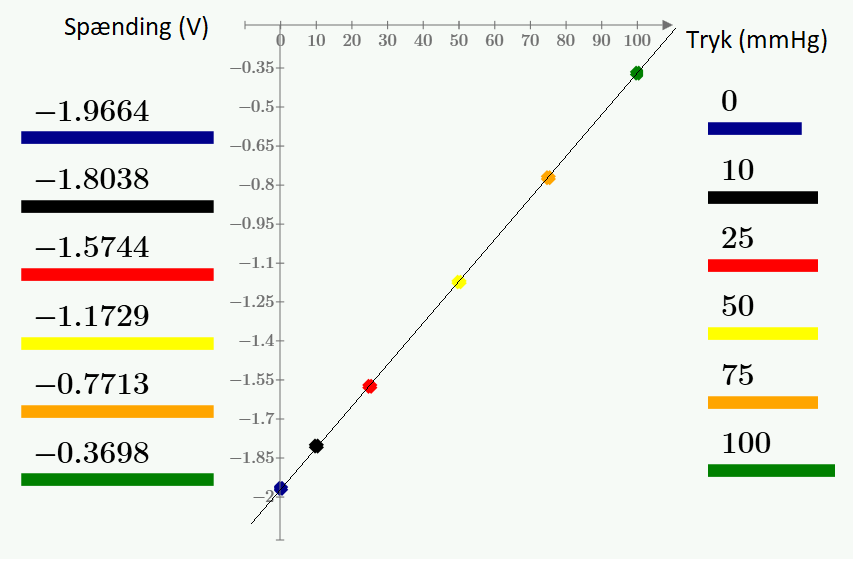
\includegraphics[width=0.8\linewidth]{../Rapport/Implementering_og_test/Hardware/integrationsplothw}
	\caption{Spænding som funktion af tryk}
	\label{fig:integrationsplot}
\end{figure}

Det ses at punkterne ligger for en lige linje, og der er derfor en god sammenhæng mellem tryk og spænding. Derudover ligger værdierne indenfor det forventede område, hvilke er -2 og 2 V, og testen gik derfor som forventet.


Ovenstående tests gav os en god indikation for, at hardwaren var velfungerende, og var klar til at blive realiseret i multisim.

\clearpage